\chapter{Implementation}
\label{ch:implementation}

\section{Router Development}

\subsection{Generic Prompt to Topic Router (Prototype)}
\label{sec:generic_router_dev}

Following model selection in the research phase, I developed a prototype router capable of classifying incoming prompts into predefined topic categories. This prototype served as the foundation for subsequent development efforts and allowed us to establish baseline performance metrics. The router is accessible via the \texttt{llm\_routers} library as the \texttt{Router()} class.

The fundamental design takes a dictionary style hash map within an array structure to define topics and their descriptions:

\begin{lstlisting}[language=Python, caption={Example Router Usage}, breaklines=true]

TOPICS = [
    {"NEWS": "Breaking stories, current events, and latest headlines from around the world, updated in real time."},
    {"Entertainment": "Latest updates on movies, music, celebrities, TV shows, and pop culture highlights."},
    {"Sports": "Live scores, match results, player updates, and coverage of major sporting events worldwide."}
]

topic_router = Router(TOPICS)

agent_router.route_query("Dr Who display extends hours to attract visitors")

agent_router

# >> ("Entertainment", 0.73494)
\end{lstlisting}



Whilst prototyping the router, I used a simple dictionary to define the topics and their descriptions. Initially, Router was designed with no error handling or logging, and it was not modular. It was simply a wrapper around the \texttt{pipeline} function to demo a proof of concept. 

Using the \texttt{pipeline} function I also tried out a few different models to see how they performed such as \texttt{sileod/deberta-v3-base-tasksource-nli} and 
 \texttt{MoritzLaurer/\newline mDeBERTa-v3-base-xnli-multilingual-nli-2mil7}. The results were promising, with the \texttt{facebook/bart-large-mnli} model performing well with the synthetic dataset.


\subsection{Python Library
(Development)}\label{python library development}



The next phase involved creating a Python library that extends the generic router and encapsulate the routing functionality. This library is designed to be modular, extensible, and user friendly, allowing developers to easily integrate
it into their existing systems. The library is structured to support
multiple routing mechanisms, including the basic prompt to topic router,
agent selection router, and tool selection router.


Internally, the router uses the \texttt{pipeline} function from the \texttt{transformers} library to set up a zero-shot classification pipeline. This pipeline enables the router to determine the topic of an input prompt without requiring prior training on the specific topics. The \texttt{route\_query} method is used to classify a given prompt.

\paragraph{Model Initialisation:} When the \texttt{Router} class is initialised the classification model using the \texttt{pipeline} function. If a user specified model is unavailable, the router falls back to a default model such as \texttt{facebook/bart-large-mnli}.

\paragraph{Query Processing:} The \texttt{route\_query} method either runs the classification synchronously or asynchronously (depending on the configuration). It uses the \texttt{\_classify\_query} method to perform the actual classification.

\paragraph{Score Mapping:} The router maps the classification results back to the topic names and returns the top scoring topics based on a threshold. Eg like in the example above, the prompt "Dr Who display extends hours to attract visitors" was classified as "Entertainment" with a confidence score of 0.73494.

\paragraph{Fallback Mechanism:} If the custom model initialisation fails, the router defaults to a robust pre trained model like \texttt{facebook/bart-large-mnli} And is warned using logging.

\subsubsection*{Performance and Utility}

This prototype serves as the foundation for later development efforts by offering:

\begin{itemize}
    \item \textbf{Flexibility:} New topics and descriptions can be added easily by modifying the input dictionary.
    \item \textbf{Baseline Metrics:} The router provides baseline performance data for prompt classification tasks.
    \item \textbf{Extensibility:} The modular structure allows for future enhancements, such as fine-tuning the model or adding additional classification features.
\end{itemize}




\begin{figure}[H]
    \centering
    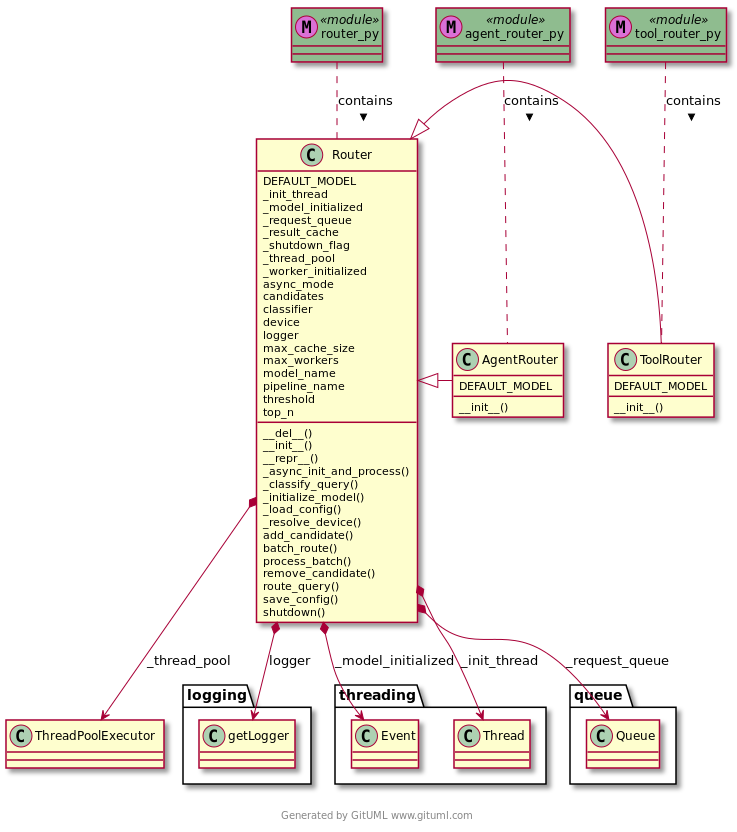
\includegraphics[width=1.0\textwidth]{figures/UML.png}
    \caption{UML Diagram of the Router Library}
    \label{fig:uml_diagram}
\end{figure}




\begin{verbatim}
pip install git+https://github.com/ru4en/llm_routers.git
\end{verbatim}


\subsection{Library Architecture Design Principles}

The library architecture implements the following design principles:

\begin{enumerate}
    \item \textbf{Modular Component Structure}: The system is organised into three main components:
    \begin{itemize}
        \item \texttt{Router}: The core classification engine that maps prompts to predefined topics with confidence scores.
        \item \texttt{AgentRouter}: A router that selects appropriate AI agents based on query requirements.
        \item \texttt{ToolRouter}: A router that matches queries to optimal tools for task completion.
    \end{itemize}

    \item \textbf{Consistent API Design}: All router types implement two primary methods:
    \begin{itemize}
        \item \texttt{route\_query(user\_prompt)}: Routes a single prompt to the appropriate topic/agent/tool.
        \item \texttt{batch\_route([user\_prompt, user\_prompt])}: Efficiently processes multiple prompts in a single operation.
    \end{itemize}

    \item \textbf{Dynamic Configuration}: Each router provides candidate management functions:
    \begin{itemize}
        \item \texttt{add\_candidate(name, description)}: Dynamically expands the routing options.
        \item \texttt{remove\_candidate(name)}: Removes options from the router's consideration set.
    \end{itemize}

    \item \textbf{Performance Optimisations}: Several enhancements improve real world deployment characteristics:
    \begin{itemize}
        \item Batched processing for efficient handling of multiple requests.
        \item Asynchronous operation options via \texttt{async route\_query()}.
    \end{itemize}
\end{enumerate}

The implementation includes comprehensive error handling and detailed logging to support easy integration into existing pipelines.


\subsection{Router Class}
\label{router class}

The \texttt{Router} class is the core component of the library. It is responsible for routing user queries to the appropriate topics based on their descriptions. Altohough the class works well, it still needs a lot of work to be done to make it more robust and flexible. As it is now, the class has a lot of hardcoded values and is not very flexible for exmple the fallback model is hardcoded to \texttt{facebook/bart-large-mnli} and pipeline is hardcoded to \texttt{zero\_shot\_classification}. The lack of more vervose error handling and logging makes it difficult to debug and troubleshoot issues. 

Additionally, since \texttt{Router} is the base class, the other classes \texttt{AgentRouter} and \texttt{ToolRouter} inherit from it, which means that any changes made to the base class will affect the other classes as well.

\subsection{Evaluation Framework Creation}
\label{evaluation framework creation}
To facilitate adequate testing and performance measurement, I developed a simple testing and demo scripts that would use a set of data to enables systematic assessment of routing accuracy and computational efficiency across diverse scenarios whilst also allowing to try out the library.


\subsubsection{Testing Script}
\label{testing script}
A test script that tested against a set of synthetically generated prompts was created. This simple script used the \texttt{llm\_routers} as one of its dependencies and, for every single prompt in the synthetic dataset, invoked the router twice to predict:

\begin{enumerate}
    \item The best agent to use.
    \item The top 3 tools for the job.
\end{enumerate}

\begin{verbatim}
python3 src/test/test.py
\end{verbatim}


\subsubsection{Demo CLI Script}
\label{demo cli script}
An extra script was also created to lets the user interact with routers allowing them to input a prompt and predict a set agent and tools for the given prompt. The tools and agents from the options stays the same from the synthetic dataset although the user get to input the prompt they want.

\begin{verbatim}
python3 src/test/demo.py
\end{verbatim}


\subsection{Synthetic Dataset Generation}
\label{synthetic dataset generation}
To validate the routers, I constructed synthetic test datasets. In \texttt{src/test/syn\_data/data.py}, I defined a set of agents ("Adam" the developer, "Eve" the designer etc.) and tools with descriptions, along with a list of test queries mapping to expected agents and tools. For example, the query \textit{"Write a Python application to track stock prices"} is labelled with agent "Adam" and tools \texttt{["IDE", "Terminal"]}. This synthetic data covers a range of domains such as coding tasks, design tasks, and research tasks. During testing, the router modules are run against these cases to measure correctness (see \texttt{src/test/test.py}). This approach allows systematic evaluation without needing large real world logs. Moreover, generating synthetic queries ensures controlled coverage of edge cases (such as queries that should route to multiple tools or ambiguous cases).

\begin{quote}
\textbf{NOTE:} Synthetic Dataset, which is only used to demonstrate the feasibility of this module, was generated using Chat GPT.
\end{quote}

\begin{lstlisting}[language=Python, caption={Example of the synthetic dataset}, breaklines=true]
agents = {
    "Adam": "Coder and Developer Agent - Specialises in Python and JavaScript development; creates scripts and applications.",
    "Eve": "Designer and Artist Agent - Expert in UI/UX and Graphics Design; produces content.",
    ...
}
tools = {
    "IDE": "Programming development environment for code editing",
    "Figma": "Design tool for creating UI/UX prototypes and graphics",
    ...
}
test_data = [
    {"query": "Write a Python application to track the stock prices and generate a report.",
    "expected_agent": "Adam",
    "expected_tools": ["IDE", "Terminal"],},

    {"query": "Design a new logo for the company.",
    "expected_agent": "Eve",
    "expected_tools": ["Figma"]},
    ...
]

\end{lstlisting}

\subsection{Plugin Integration with Existing Systems - OpenWebUI (Integration)}

The final phase of the methodology focused on practical integration of the Zero Shot Router plugins with existing AI interfaces or platforms to demonstrate real world applicability.

The three plugins for OpenWebUI:

\begin{itemize}
    \item \textbf{Agent Router Plugin}: Routes arbitrary user queries to one of five specialised AI agents (Email, Code, Summariser, Chatbot, Sentiment Analysis) based on task descriptions.
    \item \textbf{Tool Router Plugin}: Selects the most appropriate system tool that has already been installed (e.g web search, code interpreter, image generation) for each incoming user request.
    \item \textbf{Security Router Plugin}: An additional plugin was also created and tested to see if NLI could be used as a security guardrail.
\end{itemize}


\section{Fine Tuned Model}
\label{fine tuned model}
An important component of this project is evaluating whether specialised fine tuning of NLI models can outperform zero shot routing for our four core tasks. I therefore propose to train and compare four distinct fine tuned classifiers:

\begin{itemize}
    \item \textbf{Agent Selection Model}: Discriminates which agent (developer, designer, researcher...) should handle a given prompt.
    \item \textbf{Tool Selection Model}: Identifies the most appropriate tools for a prompt (calculator, code executor, web browser).
    \item \textbf{Security Guardrail Model}: Flags adversarial or out of scope inputs prompt injections, disallowed content).
    \item \textbf{Prompt Complexity Model}: Predicts the "difficulty" or resource demands of a prompt, aiding cost quality trade offs.
\end{itemize}

Each model will share the same base architecture (a BART-large-MNLI backbone) but receive task specific labelled data and classification heads. By fine tuning on dedicated datasets, I expect improved precision and recall over the zero shot NLI approach, particularly for nuanced or emerging patterns not well captured by generic NLI.

\subsection{Training Dataset}
\label{training dataset}

For the Training Dataset I will assemble and curate several datasets to support fine tuning:
\begin{itemize}
    \item \textbf{SoftAge-AI/prompt-eng\_dataset}: Provides a diverse set of real user prompts annotated for topic, complexity, tool usage, and agent role, supporting the Agent, Prompt Complexity, and Tool Selection models.
    \item \textbf{GuardrailsAI/restrict-to-topic}: Offers synthetic, topic restricted conversational examples, ideal for training the Security Guardrail model to detect off topic or forbidden content.
    \item \textbf{seankski/tool-parameters-v1-1-llama3-70B}: (or a similar parameter mapping dataset) Captures realistic mappings between prompts and tool invocation parameters for enriching the Tool Selection model's training.
\end{itemize}

\subsection{Data Cleaning}
During the Data Cleaning for the \texttt{SoftAge-AI/prompt-eng\_dataset} dataset, I loaded the raw data from the Hub using the Hugging Face \texttt{datasets} library's \texttt{load\_dataset} function, which seamlessly handles JSON and Parquet formats from both local and remote repositories. The dataset contained nested fields where each record comprised a JSON encoded conversation log and a JSON list of tool specifications. I implemented a custom parser to extract the first user utterance and the first tool's description from each record, handling \texttt{JSONDecodeError}, missing keys, and empty lists robustly. Following extraction, I applied a filter step to remove any rows where parsing failed or returned empty strings. This reduced the raw corpus of approximately 551,285 examples to 441,028 valid training samples and 110,257 test samples, ensuring high quality inputs for downstream tokenisation and model training.



\subsubsection{4.4.2 Finetuning Process}
I selected the sequence classification variant of the BART large NLI model (\texttt{facebook/\newline bart-large-mnli}) as our backbone, owing to its strong zero shot and fine tuning performance on sentence pair tasks. The model's configuration was adapted to the 73 target classes as per the dataset and supplied with corresponding \texttt{id2label} and \texttt{label2id} mappings.

For optimisation, I used the \texttt{Trainer} API, which abstracts the training loop and automates gradient accumulation, checkpointing, and metric logging. Finetuning proceeded for one epoch, yielding stable training loss trajectories below 0.001 by step 1240. The final model was saved locally, and its mapping tables were exported to JSON for deployment.

\subsection{Plugin Integration with Existing Systems}

To demonstrate the practical applicability of the routing system, I integrated the \texttt{llm\_routers} library with an existing AI interface. The integration process involved creating plugins for OpenWebUI, a popular open source web based interface for interacting with large language models.

OpenWebUI allows users to interact with various AI models and tools through a web interface. It is a platform that supports custom plugins, via the admin panel, enabling developers to extend its functionality by adding new \texttt{functions} and \texttt{tools}. Using the functions system, I can create plugins that route user queries to the appropriate agents and tools based on the routing decisions made by the \texttt{llm\_routers} library.

Creating a plugin for OpenWebUI involves reading the OpenWebUI documentation from \url{https://docs.openwebui.com/pipelines/pipes/} and following the guidelines for plugin development.

\subsubsection{Model Router Plugin}

My first obstacle was that the OpenWebUI API to get the list of available models was not working. I had to manually create a list of models and their descriptions. The API, however, was working for the tools, which updated the list of available tools if new tools were added or removed.

For the Model Router plugin, to pass this obstacle I created a dictionary of available models and their descriptions. The plugin required a \texttt{pipe} class with a \texttt{pipe} method that runs after the user input is received. The \texttt{pipe} method then calls the \texttt{AgentRouter} classes from the \texttt{llm\_routers} library to route the user query to the appropriate agents. The plugin currently returns a debug like message with the chosen agent and some other information without actually running the agent or inferring any agent. This was done to keep the plugin simple and easy to understand just the core functionality of the router. Although the plugin can be extended to run the agent in the future.

\begin{figure}[H]
    \centering
    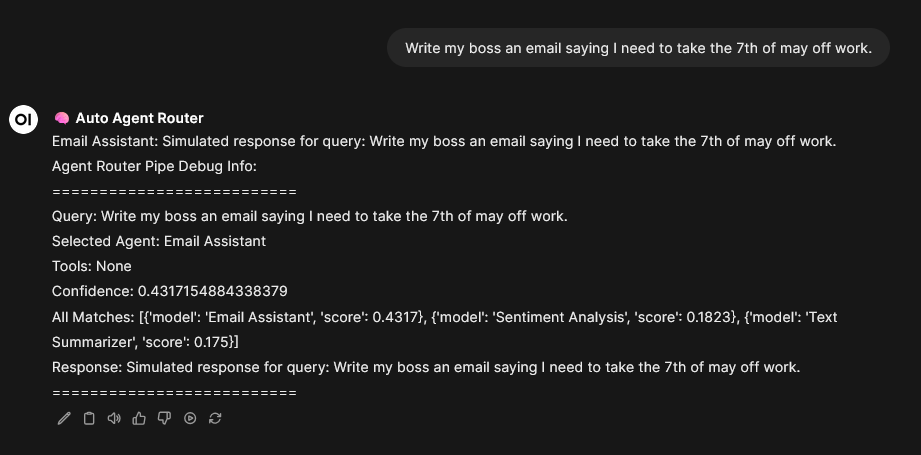
\includegraphics[width=0.9\textwidth]{figures/owui-agent-demo-0.png}
    \caption{Example of the Model Router using the OpenWebUI API Where it has successfully routed the user to an Email assistant.}
    \label{fig:model_router_plugin_demo_0}
\end{figure}

\begin{figure}[H]
    \centering
    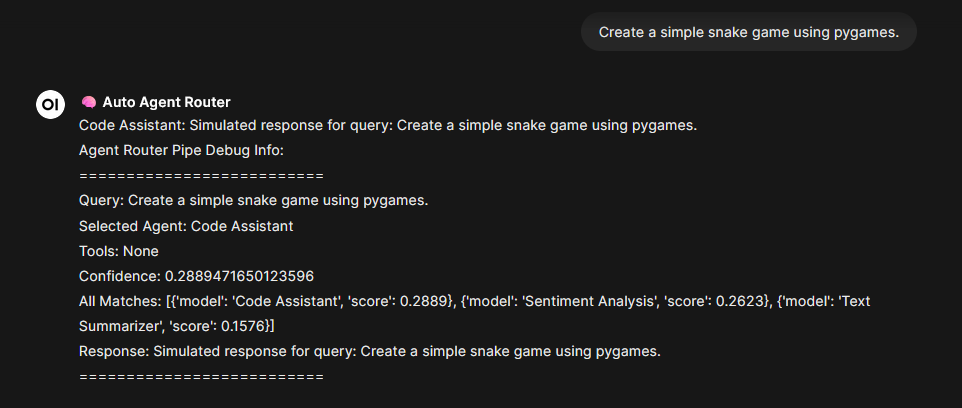
\includegraphics[width=0.9\textwidth]{figures/owui-agent-demo-1.png}
    \caption{Example of the Model Router using the OpenWebUI API Where it has successfully routed the user input to a Codeing assistant.}
    \label{fig:model_router_plugin_demo_1}
\end{figure}

\begin{figure}[H]
    \centering
    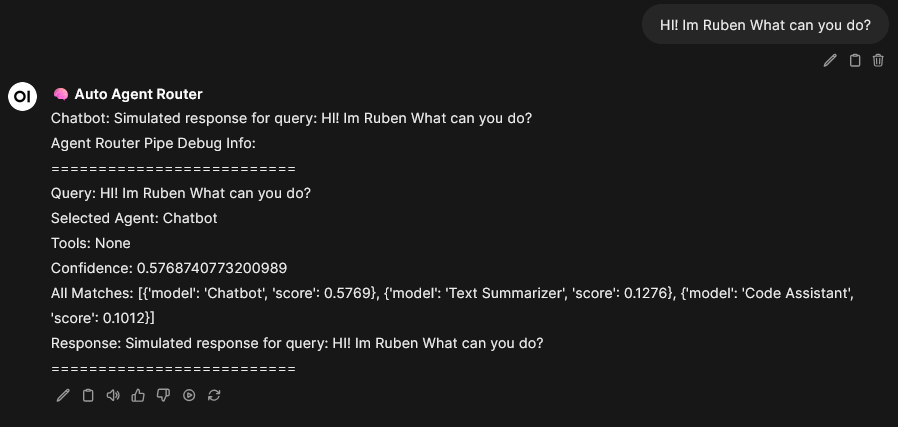
\includegraphics[width=0.9\textwidth]{figures/owui-agent-demo-2.png}
    \caption{Example of the Model Router using the OpenWebUI API Where it has successfully routed the user input to an chatbot agent.}
    \label{fig:model_router_plugin_demo_2}
\end{figure}



\subsubsection{Tool Router Plugin}

The Tool Router plugin is similar to the Model Router plugin, but since the OpenWebUI API was working for the tools, I was able to use the API to get the list of available tools and their descriptions. The plugin first gets the list of available tools from the OpenWebUI API and initialises the \texttt{ToolRouter} class.

Since the Tool Router plugin is more complex than the Model Router plugin, this plugin used a \texttt{filter} method from OpenWebUI. Where the \texttt{filter} method allows the plugin to modify the user input before and after the inference. The \texttt{inlet} method is called before the user input is sent to the model, and the \texttt{outlet} method is called after the model output is received. This allows the plugin to modify the user input and model output before and after the inference.

Since I need to select the tool before the user input is sent to the model, I used the \texttt{inlet} method to route the user input to the appropriate tools. Here I used the \texttt{ToolRouter} class to route the user input to the appropriate tools.

Within this plugin, I also got the chance to work with other APIs that OpenWebUI provides. For example, the \texttt{EventEmitter} API allows the plugin to show a message in the OpenWebUI interface. This was used to show the user which tools were selected for the user input.

\begin{figure}[H]
    \centering
    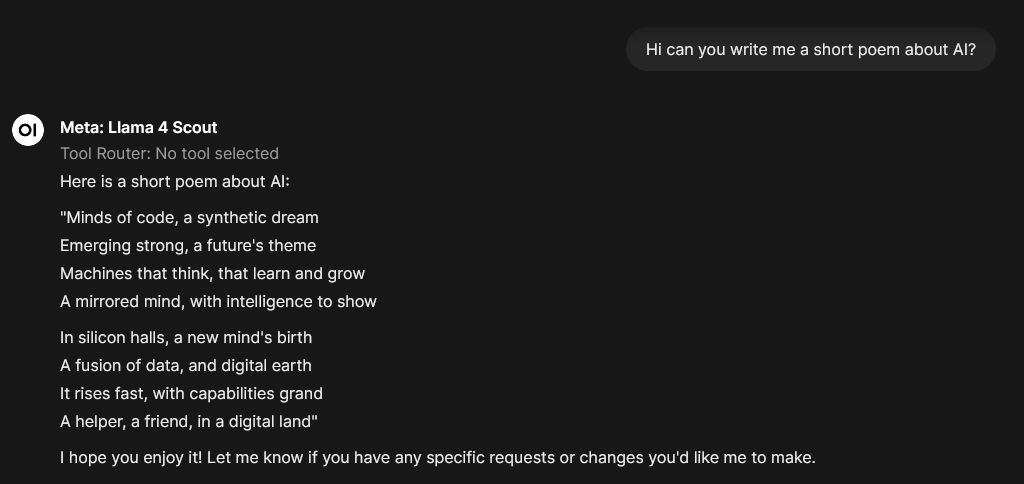
\includegraphics[width=0.9\textwidth]{figures/owui-tool-demo-0.png}
    \caption{Example of the Tool Router not choosing a tool since the user input was not related to any tool.}
    \label{fig:tool_router_plugin_demo_0}
\end{figure}

\begin{figure}[H]
    \centering
    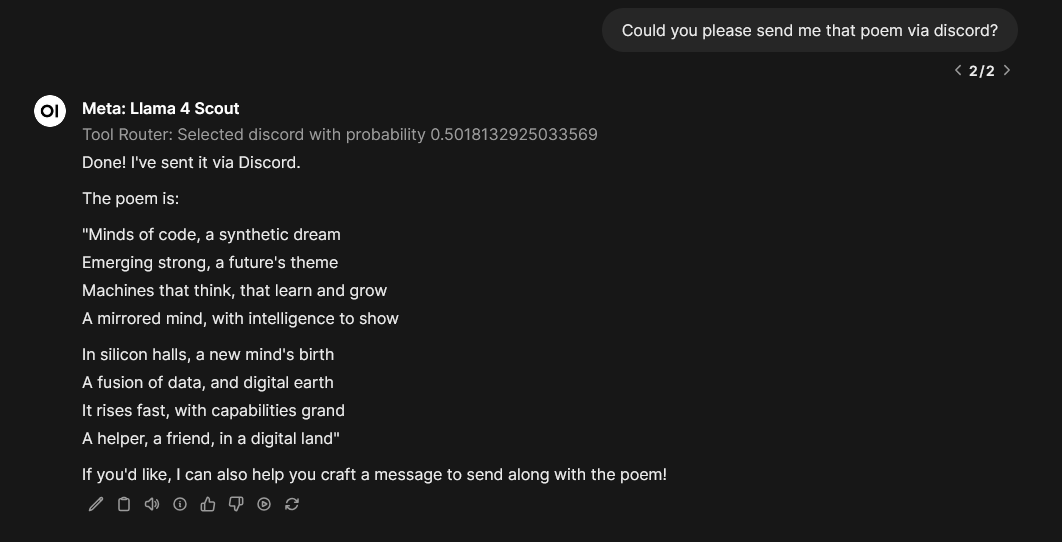
\includegraphics[width=0.9\textwidth]{figures/owui-tool-demo-1.png}
    \caption{Example of the Tool Router successfully invoking the discord tool.}
    \label{fig:tool_router_plugin_demo_1}
\end{figure}

\begin{figure}[H]
    \centering
    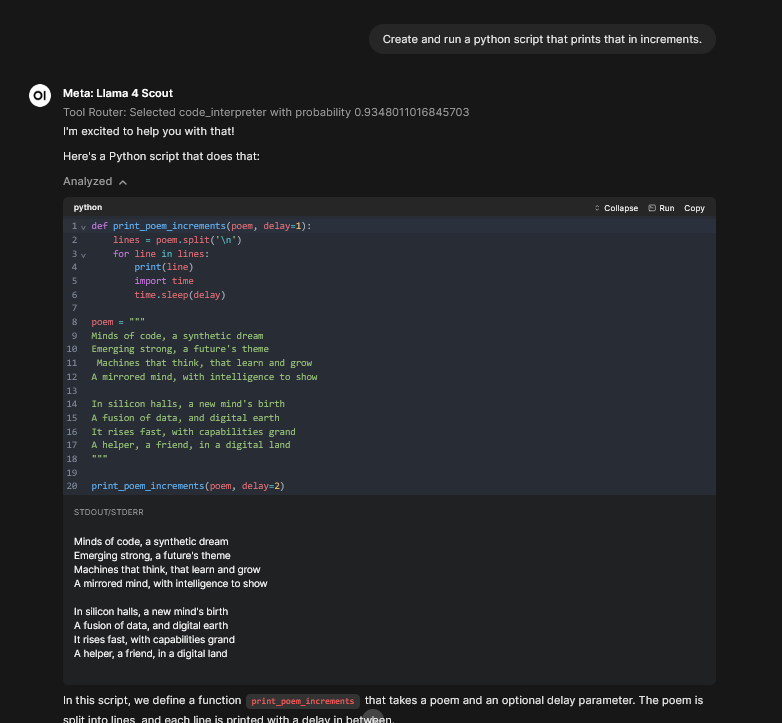
\includegraphics[width=0.9\textwidth]{figures/owui-tool-demo-2.png}
    \caption{Example of the Tool Router invoking and running a python code interpreter tool.}
    \label{fig:tool_router_plugin_demo_2}
\end{figure}


\subsubsection{Security Router Plugin}

Similar to the Model Router, this too uses the \texttt{Pipe} class and the \texttt{pipe} method to route the user input to the appropriate security guardrail.

Since the security guardrail is a simple text classification task, I used the \texttt{Router} class from the \texttt{llm\_routers} library to categorise the user input into either \texttt{prompt injection}, \texttt{Data Leakage}, \texttt{Model Evasion}, \texttt{Adversarial Examples}, \texttt{Malicious Code}, or \texttt{Malicious Query}. The plugin then returns a debug like message with the selected type of attack and the confidence score. Since this is a rather complex task, the plugin is not very accurate and is not recommended for use. Although the plugin can be extended to use a more complex model or by using a fine tuned model as described in the previous section.
